\documentclass{standalone}
\usepackage{tikz}
\usetikzlibrary{calc,positioning,shapes,decorations.pathmorphing}
\usetikzlibrary{hobby} % for blobs, see http://tex.stackexchange.com/a/145276

\def\gridopacity{100}
\def\gridopacity{0}

\begin{document}%
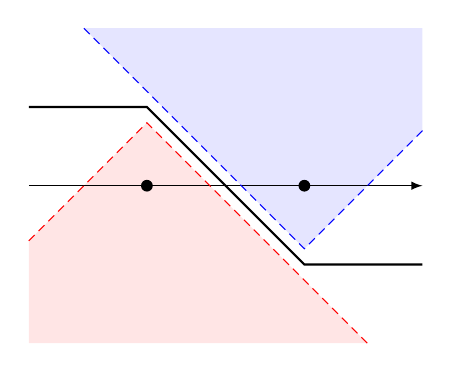
\begin{tikzpicture}
\tikzset{>=latex} % arrow heads
\draw[step=1,black!15,very thin,opacity=\gridopacity] (0,0) grid (5,4);

   \fill[blue!10] (0.7,4.0) -- (3.5,1.2) -- (5.0,2.7) -- (5.0,4.0) -- cycle;
   \fill[red!10] (0.0,1.3) -- (1.5,2.8) -- (4.3,0.0) -- (0,0) -- cycle;

   \draw[->] (0.0,2) -- (5.0,2);

   \node[fill=black,circle,inner sep=1.5pt] at (1.5,2) {};
   \node[fill=black,circle,inner sep=1.5pt] at (3.5,2) {};

   \draw[densely dashed,blue] (0.7,4.0) -- (3.5,1.2) -- (5.0,2.7);
   \draw[densely dashed,red]  (0.0,1.3) -- (1.5,2.8) -- (4.3,0.0);
   \draw[thick] (0,3.0) -- (1.5,3.0) -- (3.5,1.0) -- (5.0,1.0);

\end{tikzpicture}%
\end{document}
